%
% Another appendix chapter
\chapter{Application: Walking}\label{chap:walking}
The control strategy for a static, standing case presented in the previous chapter is two-dimensional. If the robot is walking, the horizontal \ac{CoM} position can be located outside the support polygon. The result of this is that the desired \ac{CoP} cannot always be placed in line with the \ac{ICP} error.  In this chapter, the bang-bang control law of Chapter \ref{chap:standing} is extended for the use while the robot is walking.
% Experimental Setup
\section{Experimental Setup}
In this section, to determine when to activate a similar bang-bang control law as in the previous chapter,  tests are conducted preliminary to developing a controller. In the tests, a push is applied in the beginning of single support while the robot is walking. The stepping parameters used for the tests are given in Table \ref{tab:stepping}, which are the default stepping parameters while testing in simulation. In \figref{fig:valwalkingtest}, the test setup in simulation is shown. The limited foothold options display that footstep location adjustment is not available as a balance strategy and that other balance strategies, such as \ac{CoM} height variation, might be needed to recover. In \figref{fig:3foot}, the \ac{ICP} reference trajectory, the \ac{CMP} reference trajectory and the measured \ac{CoM} trajectory, are made visible for foot hold where the push will be applied. 
\begin{table}
\caption{Stepping parameters for the walking tests.} % title of Table
\centering % used for centering table
\begin{tabular}{c c c } % centered columns (4 columns)
\hline\hline %inserts double horizontal lines
Parameter & Value & Unit \\
%heading
\hline % inserts single horizontal line
Step Legth & 0.5 &  [m]\\
Step Width & 0.25 & [m]\\
Single Support Time & 0.6 & [s]\\
Double Support Time & 0.25 & [s]\\
%[1ex] % [1ex] adds vertical space
\hline %inserts single line
\end{tabular}
\label{tab:stepping} % is used to refer this table in the text
\end{table}
\begin{figure}[h]
\centering
  \includegraphics[width=.8\linewidth]{STYLESTUFF/valwalkingtest.png}
   \caption{Test setup for push recovery during walking in simulation. The limited foothold options show that footstep adjustment is not available as a balance strategy.}
    \label{fig:valwalkingtest}
\end{figure}
\begin{figure}[h]
\centering
  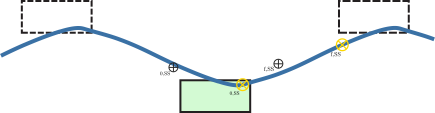
\includegraphics[width=.8\linewidth]{STYLESTUFF/ICPplan3StepComICPrSS.png}
   \caption{Trajectories during single support in the horizontal plane (gray dotted lines). The gray area is the current, right, footstep position where the push will be applied.}
    \label{fig:3foot}
\end{figure}
%Preliminary observations

The following properties are observed, when applying pushes in different directions in the start of single support:
\begin{enumerate}
	\item The direction of the \ac{ICP} error stays often approximately the same until transition to double support.
	\item If the \ac{ICP} error is directed in the sagittal plane, the desired \ac{CMP} often remains somewhat in the same location.
	\item If the \ac{ICP} error is directed  in the coronal plane, the desired \ac{CMP} slides from back to the front of the foot.
	\item The configuration and velocity near transition to double support affects the robots ability to put its swing leg down at the desired time. 
\end{enumerate}
These properties are used as assumptions in the development of a control law.
% Methods
\section{Method}
The control law of the previous chapter is first adjusted for desired \ac{CMP} positions outside the support polygon to make a high-level comparison with angular momentum strategies. Second, control variables are introduced. Third, control actions are presented, which are activated based on violation of thresholds of the presented control variables.

\subsection{Avoiding Generating Additional Angular Momentum Rate}
In the previous chapter, $\rcmpd$ is constrained to be inside the support polygon. Therefore, this point is assumed to coincide with $\rcopd$. In this section, the computation of desired linear momentum rate is adjusted for $\rcmpd$ location outside the support polygon. If $\rcmpd$ is outside the polygon, $\rcopd$ is obtained by projecting $\rcmpd$ on the polygon edge. For compatibility with the default setup, the goal is to request little to no additional angular momentum rate from the robot to achieve the desired linear momentum rate. Therefore, the vertical motion controller generates an added desired linear momentum rate on top of the default controller if $\rcmpd$ is outside the support polygon. First, the desired horizontal linear momentum rate of change, as used in the previous chapter, is written in terms of the $\rcopd$. The assumption is made that the difference in body torque $\taucom$ is directly related to the difference between $\rcmpd$ and $\rcopd$:
\begin{align}
    \dotldxy &= \frac{\cxy-\rcmpd}{z}(mg+\dotldz),\\
&=\frac{\mathbf{c}_{xy}-\Big(\rcopd+\frac{\taucom}{(mg+\dotldz)}\Big)}{z}(mg+\dotldz), \\
&=\frac{\mathbf{c}_{xy}-\rcopd}{z}(mg + \dotldz)- \frac{\taucom}{z}.
\end{align}
Writing $\taucom$ in $\rcmpd$ again, but only for the \ac{LIP} part of this equation (and assuming a constant height $z_0$ for this part), gives the following expression:
 \begin{equation}
\dotldxy = \underbrace{ \frac{\mathbf{c}_{xy}-\mathbf{r}_{cmp,d}} {z_0}mg}_{\dotldxylip}  + \underbrace{\frac{\mathbf{c}_{xy}-\mathbf{r}_{cop,d}}{z}\dotldz}_{\dotldxyheight},
\end{equation}
where $\dotldxyheight$ is the additional desired horizontal linear momentum rate from the vertical motion controller and $\dotldxylip$ the desired momentum rate from the default control law.

In Figure \ref{fig:rcopdvsrcmpd}, it is visually explained how this computation of $\dotldxy$ will not require additional angular momentum rate from the robot, as the scalar offset $a$ in the figure is the same for both setups. If \ac{CoM} height variation would be used based on the location of $\rcmpd$, additional angular momentum rate would be needed about the \ac{CoM} to achieve the desired linear momentum rate. However, using this modified desired linear momentum rate with both $\rcmpd$ and $\rcopd$, the resulting \ac{CMP} will be different then $\rcmpd$, as shown in the image. 

\begin{figure}
\centering
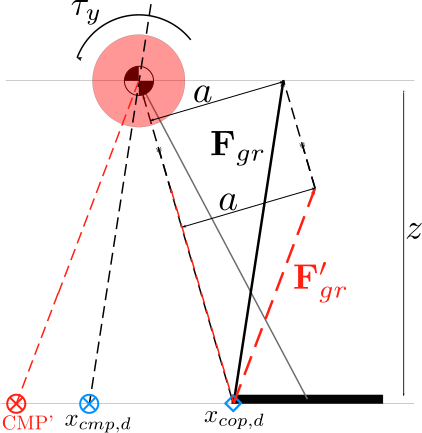
\includegraphics[width=0.45\textwidth]{STYLESTUFF/2DControlStrategyViz.png}
\caption{Explanatory drawing of the \ac{GRF} resulting from the default desired momentum rate (black) versus the modified desired momentum rate for \ac{CoM} height variation (red). The thin arrows show the part of the \ac{GRF} that intersects with the \ac{CoM}, which is used for height changes. The equal scalar offset $a$ shows that the same angular momentum rate will be requested about the \ac{CoM}.}
\label{fig:rcopdvsrcmpd}
\end{figure}
\subsection{Alignment Angle and Effective Distance}
If the \ac{CoM} is outside the support polygon, the local virtual leg between $\rcopd$ and the horizontal \ac{CoM} location $\cxy$ may not be aligned with direction of the \ac{ICP} error $\icpe$. This results in the leg applying force in a different direction than is desired to cancel the error, which can result in additional error in another direction. Also, if $\cxy$ is close to the polygon edge, the distance with $\rcopd$ might be very small, such that height changes have little to no effect as the local \ac{VHIP} is close to upright. To take these two aspects into account, the following variables are introduced, which will be used to determine when to use \ac{CoM} height variation for balance:
\begin{itemize}
	\item \textbf{Alignment angle} $\phi$: the angle between the virtual leg $\rcopd-\cxy$ and the \ac{ICP} error $\icpe$;
	\item \textbf{Effective distance} $\delta$: the distance between $\rcopd$ and $\cxy$ in the direction of the \ac{ICP} error $\icpe$.
\end{itemize}

In \figref{fig:phiViz}a-b, the two variables are graphically explained using the stance foot position and configuration of \figref{fig:3foot}. The desired \ac{CMP} $\rcmpd$ is allowed to move a small distance outside the polygon. In \figref{fig:phiVizc}, the angle $\phi$ is zero and the distance $\delta$ is relatively large. This is a relatively suitable error for height control, as the alignment angle is aligned and the local \ac{VHIP} tip is relatively far from the base. In \figref{fig:phiVizd}, the angle $\phi$ is $90$ degrees and therefore the distance $\delta$ is zero. In this configuration, \ac{CoM} height variation would not help drive the error back. Furthermore, an additional error would occur orthogonal to the current $\icpe$. Therefore, this error is not considered suitable for using \ac{CoM} height variation for balance control.
\begin{figure}[h]
\centering
  \begin{subfigure}{0.49\textwidth}
    \centering
  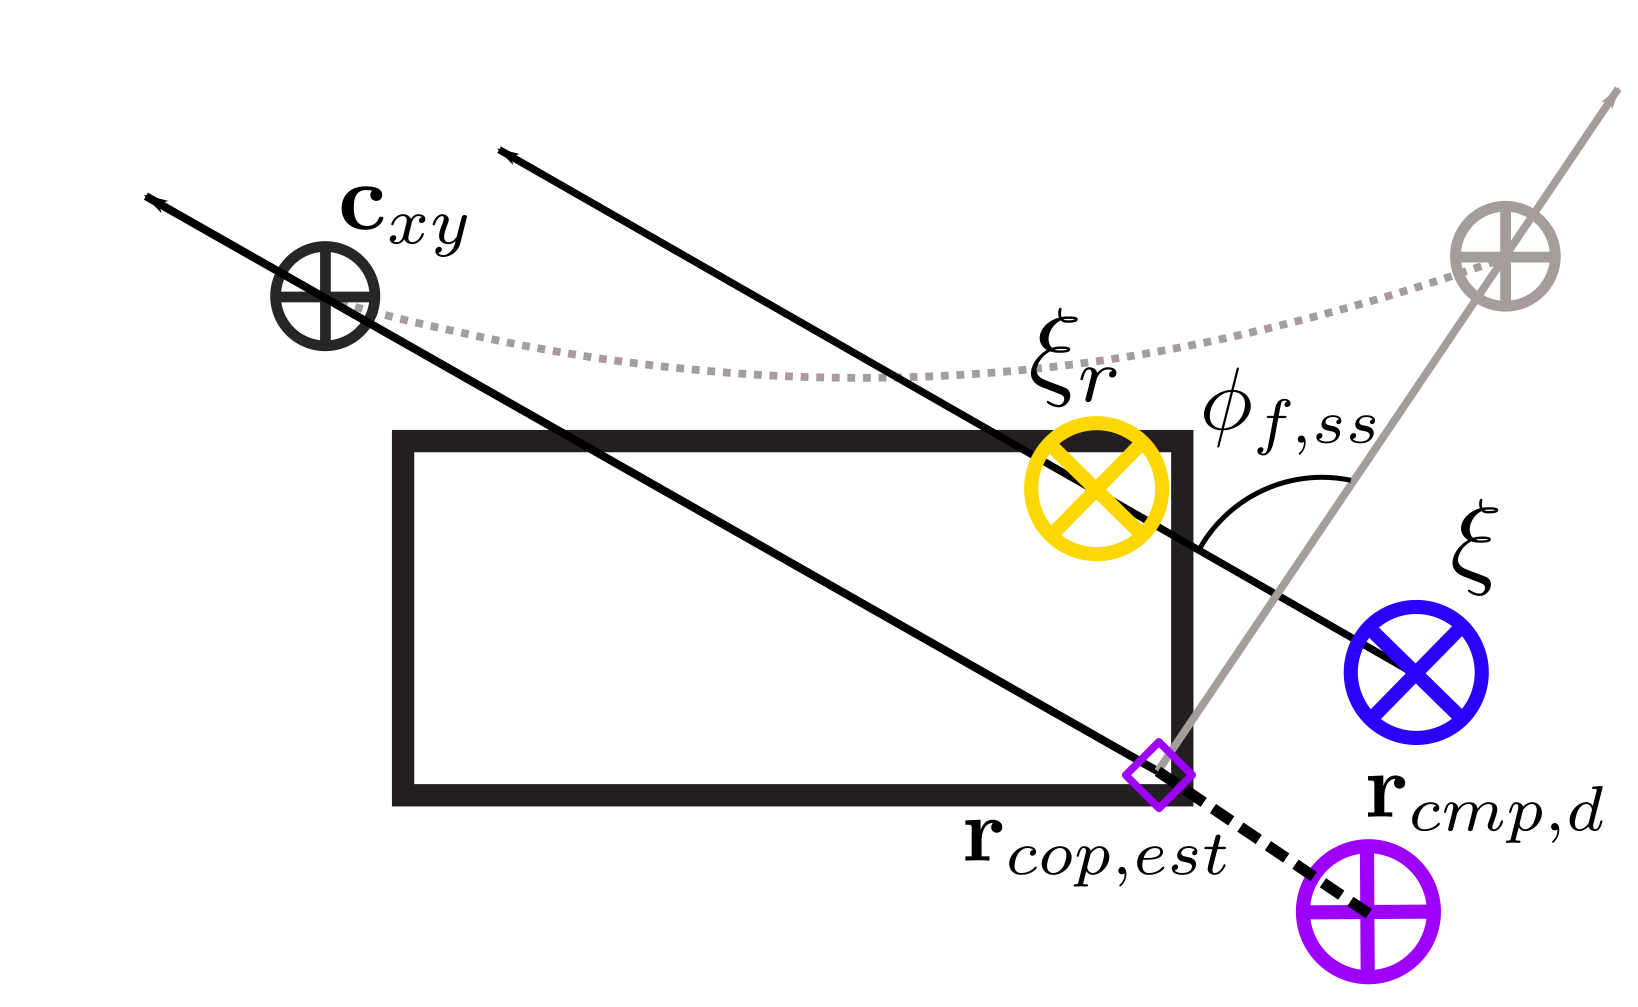
\includegraphics[width=.7\linewidth]{STYLESTUFF/ICPplanStartSSPhiViz0.png}
    \caption{}
     \label{fig:phiVizc}
  \end{subfigure}
  \begin{subfigure}{0.49\textwidth}
    \centering
  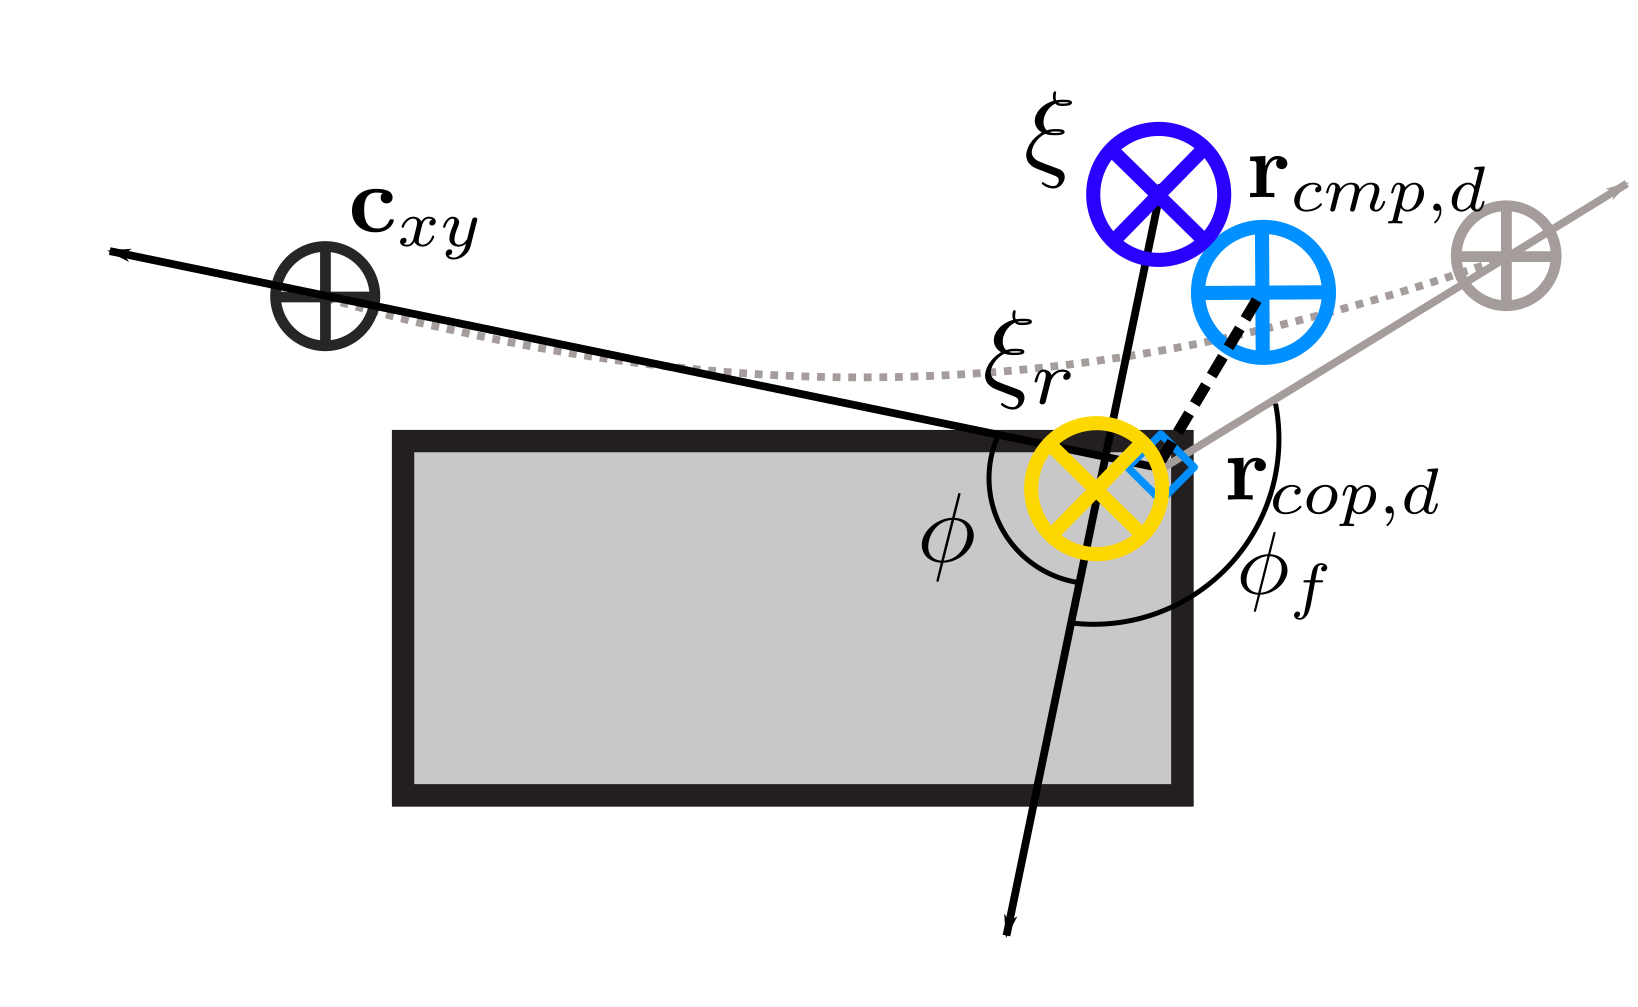
\includegraphics[width=.7\linewidth]{STYLESTUFF/ICPplanStartSSPhiViz90.png}
    \caption{}
     \label{fig:phiVizd}
  \end{subfigure}
  \begin{subfigure}{0.49\textwidth}
  \centering
  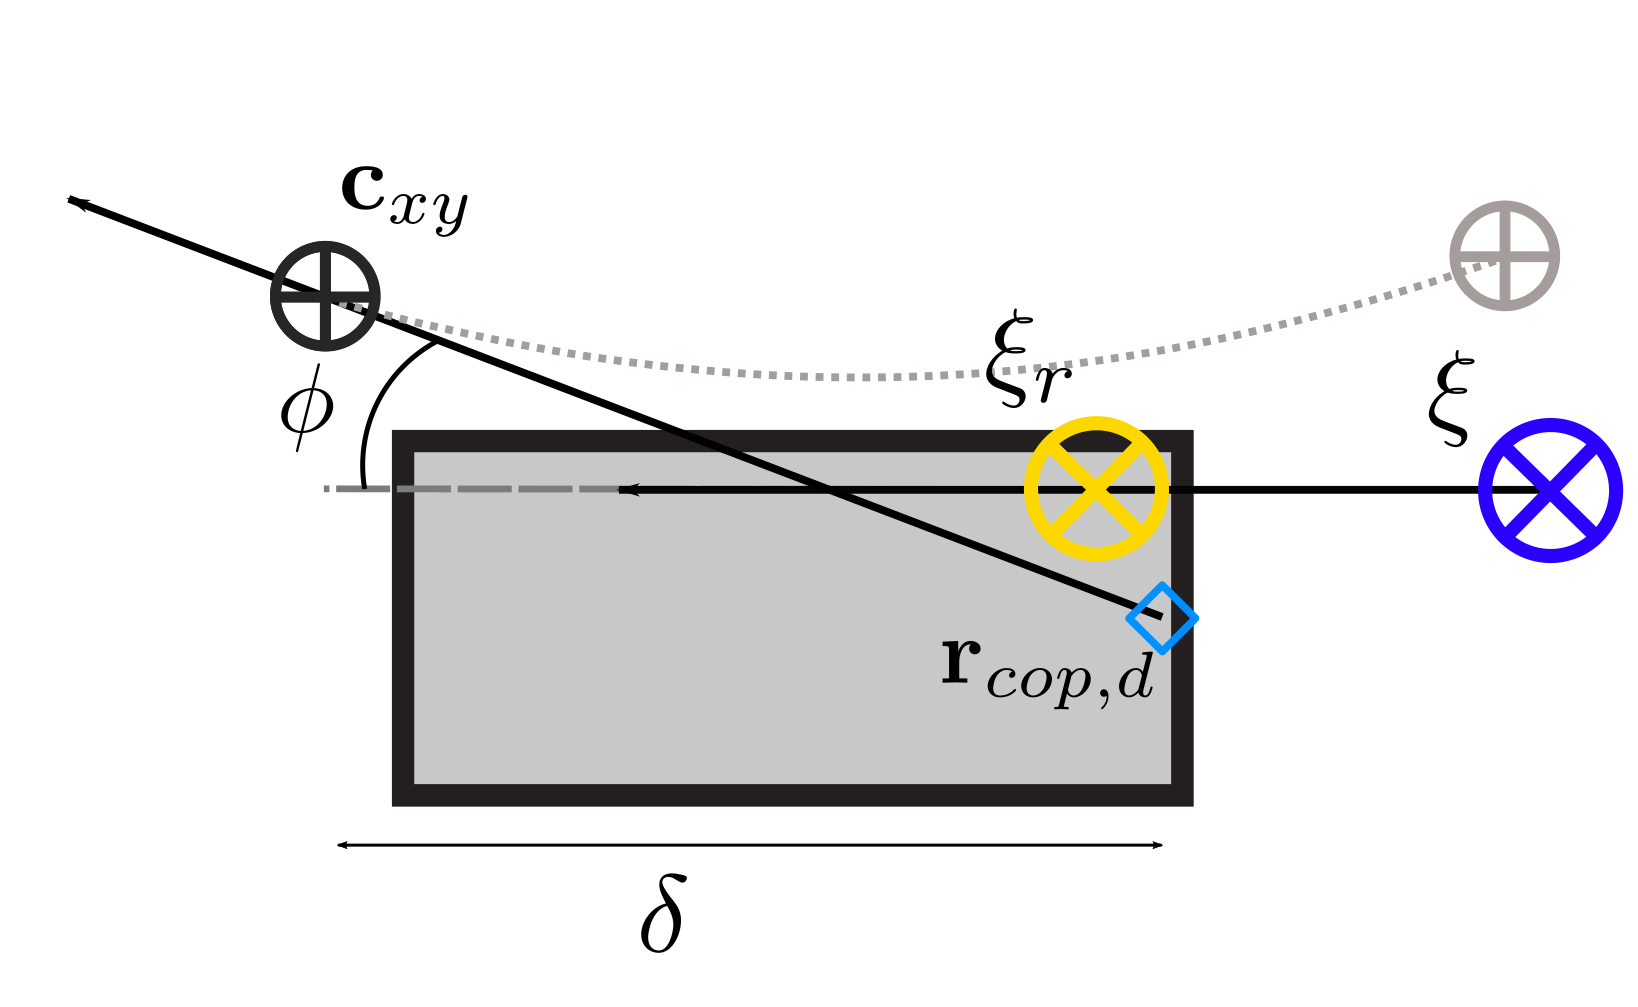
\includegraphics[width=.7\linewidth]{STYLESTUFF/ICPplanStartSSPhiVizNegError.png}
   \caption{}
    \label{fig:phiViza}
  \end{subfigure}
  \begin{subfigure}{0.49\textwidth}
    \centering
  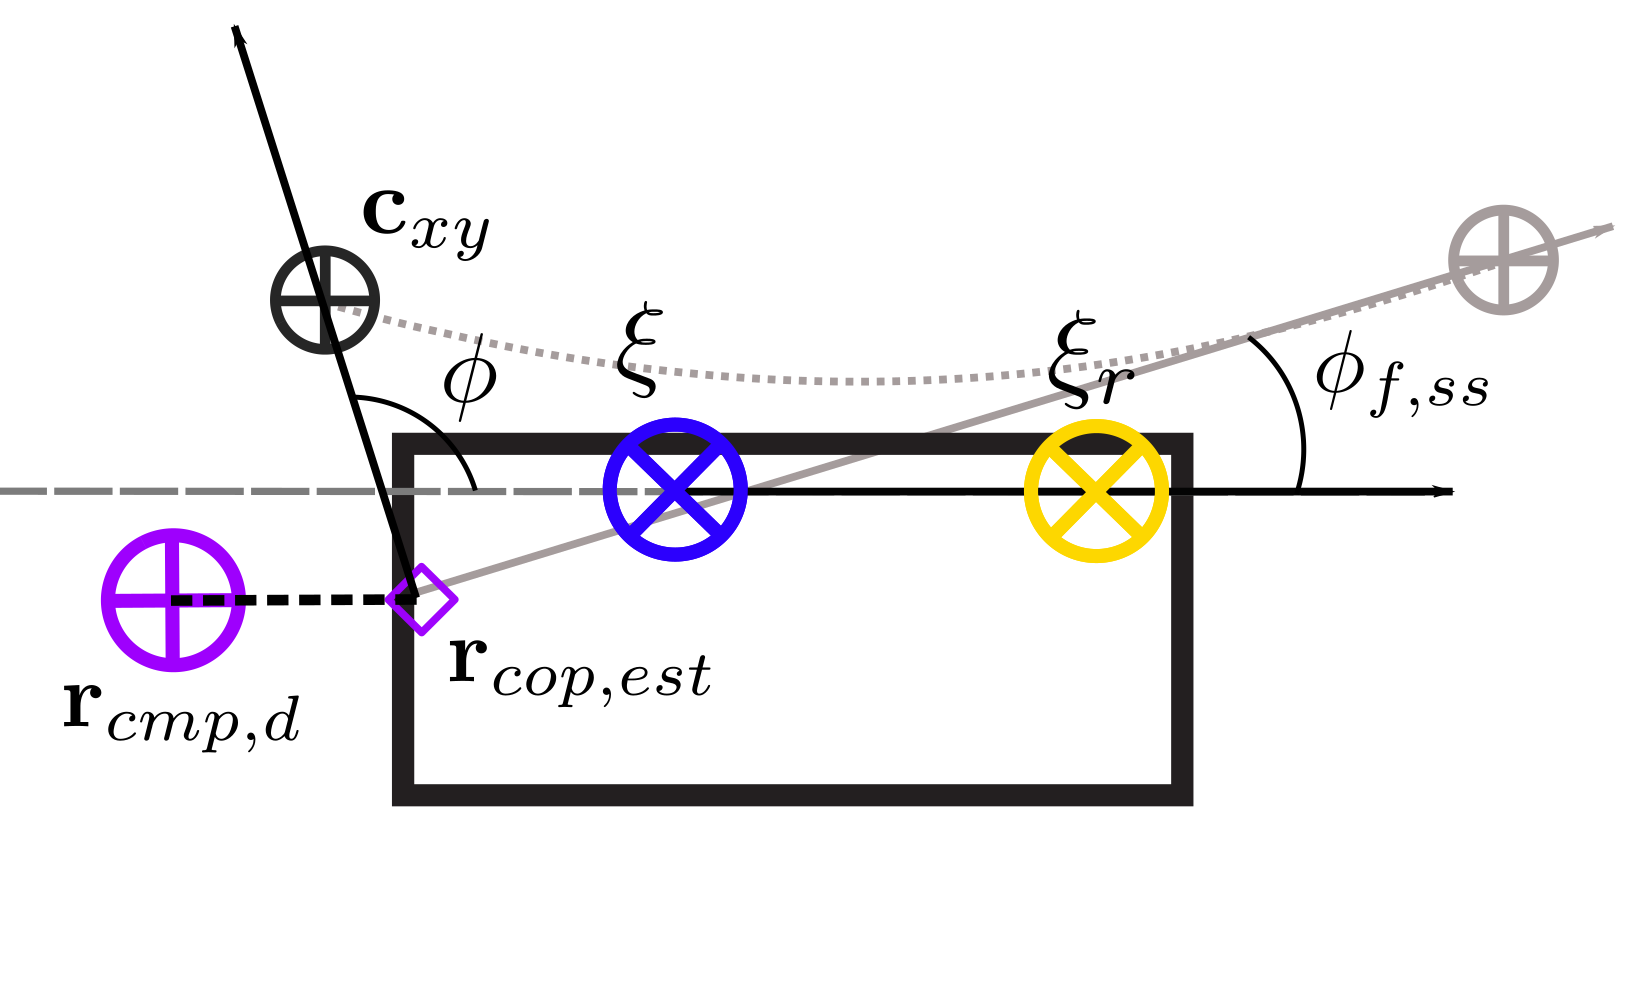
\includegraphics[width=.7\linewidth]{STYLESTUFF/ICPplanStartSSPhiViz.png}
  \caption{}
   \label{fig:phiVizb}
  \end{subfigure}
    \begin{subfigure}{0.49\textwidth}
    \centering
  \includegraphics[width=.7\linewidth]{STYLESTUFF/ICPplanStartSSPhiVizLeftError.png}
    \caption{}
     \label{fig:phiVize}
  \end{subfigure}
  \begin{subfigure}{0.49\textwidth}
    \centering
  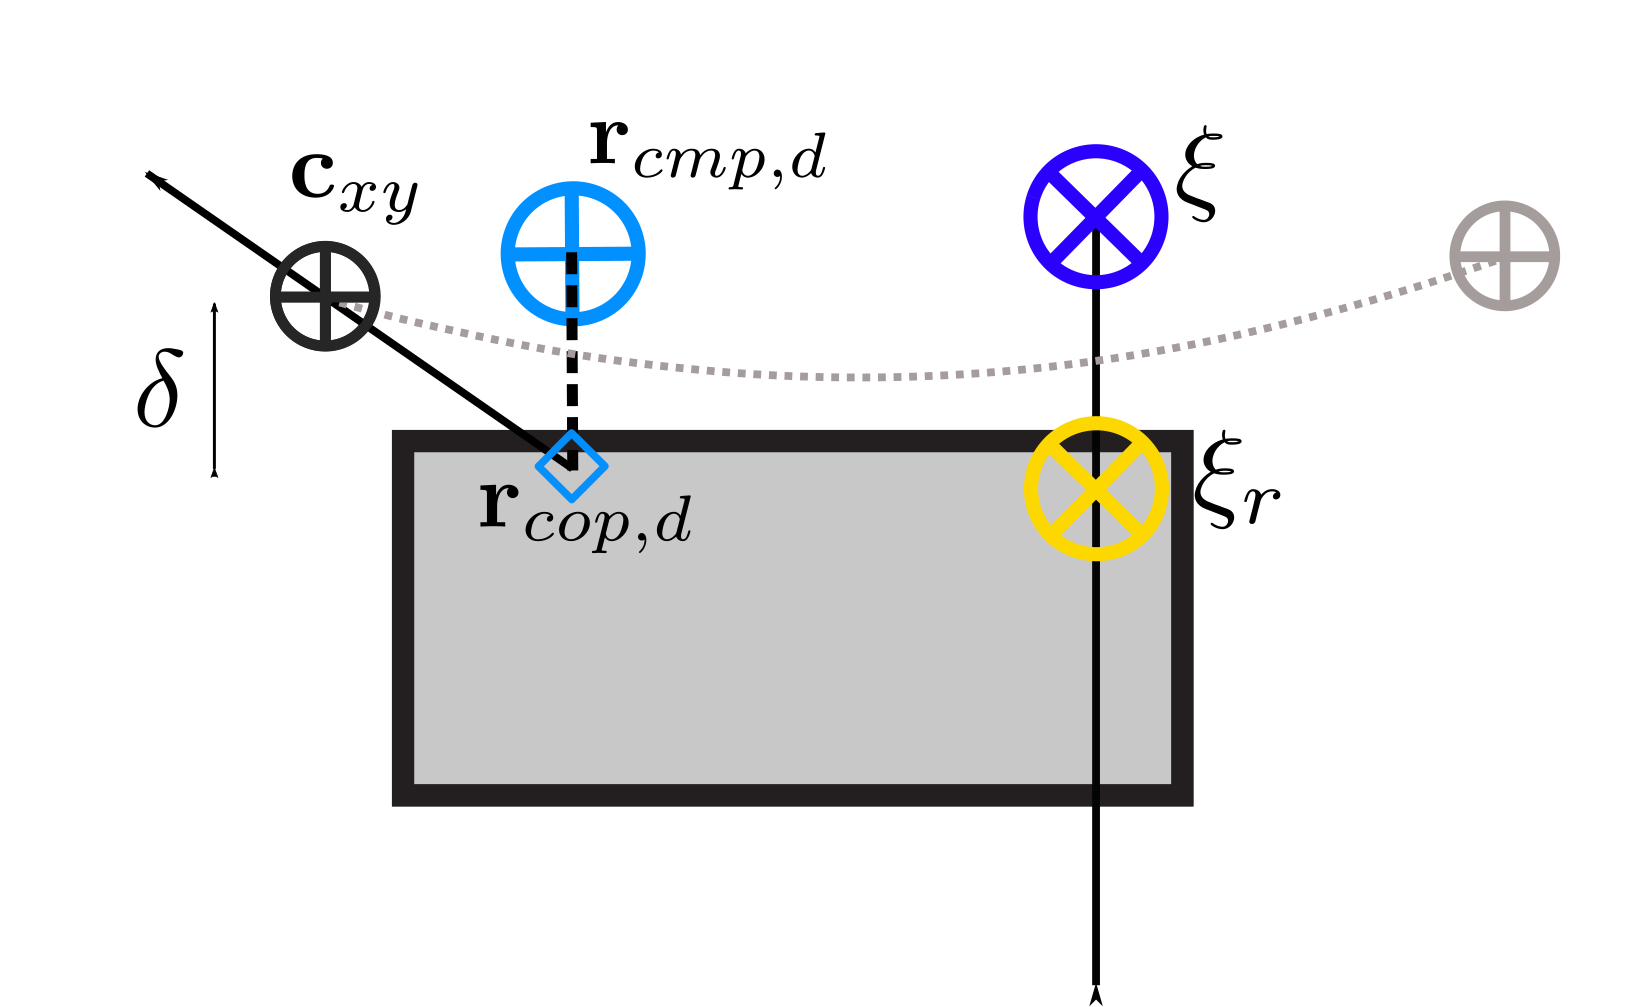
\includegraphics[width=.7\linewidth]{STYLESTUFF/ICPplanStartSSPhiVizRightError.png}
    \caption{}
     \label{fig:phiVizf}
  \end{subfigure}
  \caption{Explanatory visualizations of $\phi$ and $\delta$ for the configuration at start of single support with different \ac{ICP} error directions.}
  \label{fig:phiViz}
\end{figure}

\subsection{Actions}
The alignment angle $\phi$ and the effective distance $\delta$ are used to select a control action if a minimum threshold for $\icpe$ is met, like in the previous chapter. From the assumptions of the preliminary observations $1$ and $2$, it is assumed that the angle $\phi$ will be dependent on the current $\icpe$ and $\rcopd$ throughout single support if $\icpe$ is directed in the sagittal plane. Therefore, the additional variables $\delta_f$ and $\phi_f$ are used, which are the expected alignment and distance in the end of single support, based on the planned \ac{CoM} location coming from the \ac{ICP} planner. Also, from assumption $3$, $\phi$ is not used if a push is in the coronal plane, because throughout single support the foot length is available for future $\rcmpd$ placements that could correct any additional error. Based on the discussed variables, the following three actions can be selected:
\begin{itemize}
	\item \textbf{Positive alignment}: At the current control tick, $\phi$ is relatively aligned and $\delta$ relatively large for a push in the sagittal plane, or $\delta$ is relatively large for a push in the coronal plane. Also, $\phi$ has to be smaller than $\frac{1}{2}\pi$ [rad], as the virtual leg must be in direction of the \ac{ICP} error to make additional force effective. A bang-bang action is activated, similar to the control law of the previous chapter. The thresholds related to this action are $\phimin < \phi < \phimax$ (for a push in the sagittal direction) and $\delta > \deltamin$, where $\phimin$, $\phimax$ and $\deltamin$ are parameters for the minimum and maximum $\phi$ and minimum $\delta$.
	\item \textbf{Prepare}: At the current control tick, $\phi$ is relatively misaligned or $\delta$ is relatively small, but $\phi_f$ and $\delta_f$ are at values suitable for the positive alignment action. The \ac{CoM} height is gradually lowered to the minimum height, after which a positive `bang' is used. The the thresholds related to this action are $\phimin<\phi_f<\phimax$ and $\delta_f>\deltamin$.
	\item \textbf{Default}: All decisions variables $\phi$, $\delta$, $\phi_f$ and $\delta_f$ are at such values that vertical \ac{CoM} motion does not improve recovery. The default height control law is used and no additional height changes are considered. The threshold related to this action is if the prepare or the positive alignment thresholds do not hold.
\end{itemize}

In \figref{fig:phiViz}, six cases of \ac{ICP} errors are shown to explain which actions will be used. In \figref{fig:phiVizc}, the positive alignment action is used, as the $\delta$ is relatively large and $\phi$ relatively small. In \figref{fig:phiVizd}, the default action is introduced, as $\delta$ is zero and $\phi$ is misaligned. In \figref{fig:phiViza}, the error is a result of a back push. A positive alignment action is introduced, as $\phi$ is relatively small and $\delta$ relatively large. In \figref{fig:phiVizb}, a push is applied frontally on the robot. The prepare action is used, as $\delta_f$ and $\phi_f$ are more suitable for height control. In \figref{fig:phiVize}, the robot is pushed from the left. The positive alignment action is used, as the current $\delta$ is relatively large. In \figref{fig:phiVizf}, the error is a result from a push from the right. The default action is activated, as $\delta$ is small throughout single support.

The bang-bang control law considered in the actions is similar to the control law of the previous chapter. However, height constraints are slightly modified. For the maximum height constraint $\zmax$, the same constant parameter as for the standing tests is used in the first half of single support. In the second half, the maximum height constraint is linearly interpolated between the maximum height constraint for standing and a maximum height constraint at the end of single support.  For the minimum height constraint $\zmin$, a constant value is considered throughout single support. The height constraints are visually explained in \figref{fig:heightconstraints}.
\begin{figure}
\centering
  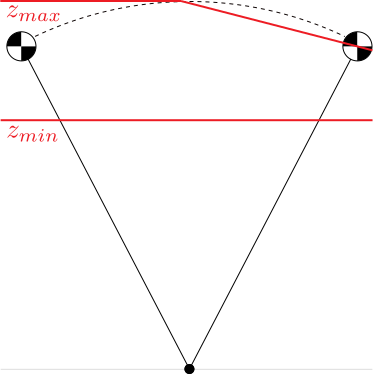
\includegraphics[width=.4\linewidth]{STYLESTUFF/heightconstraints.png}
   \caption{Height constraints through single support for the vertical motion controller while the robot is walking.}
    \label{fig:heightconstraints}
\end{figure} 
\subsubsection{Positive Alignment Action} 
Using $\zmax$ as specified above, a similar bang-bang control law as in the previous chapter is introduced with the positive alignment action. After the second `bang', the height is not controlled to the maximum height $\zmax$, but is given a feedforward downward acceleration computed from a circle around the ankle. Using the circle acceleration, the swing leg singularity can be approximated and the downward velocity at touchdown will not be as high as after a free fall. This is done to avoid singularity of the stance leg, and the swing leg at touch down. Consider the distance from the ankle of the robot to the sagittal \ac{CoM} position $x_{ankle}$ and the maximum leg length $l_{max}$. If is assumed that the \ac{CoM} height $z$ is located at the hip, the horizontal position relates to the vertical position as:
\begin{equation}
z^2 = l_{max}^2-x_{ankle}^2.
\end{equation}
The vertical velocity resulting from this function reads as:
\begin{equation}
 \dot{z} = -\frac{x_{ankle}\dot{x}}{\sqrt{l_{max}^2-x_{ankle}^2}}.
\end{equation}
The resulting vertical acceleration reads as:
\begin{equation}
\ddot{z} = \frac{\sqrt{l_{max}^2-x_{ankle}^2}(-\dot{x}^2-x_{ankle}\ddot{x}) - \frac{x_{ankle}^2\dot{x}^2}{\sqrt{l_{max}^2-x_{ankle}^2}}}{ l_{max}^2-x_{ankle}^2}.
\end{equation}
Assuming the sagittal acceleration $\ddot{x}$ is zero, the desired vertical acceleration is computed as:
\begin{equation}
 \ddzd = -\frac{\dot{x}^2}{\sqrt{ l_{max}^2-x_{ankle}^2}} - \frac{x_{ankle}^2\dot{x}^2}{(l_{max}^2-x_{ankle}^2)^{1\frac{1}{2}}}.
\end{equation}
\subsubsection{Prepare Action} 
When the future errors are more suitable for using vertical \ac{CoM} motion for balance, the \ac{CoM} height is prepared for applying more force later and therefore lowered. The control action uses the time it takes to accelerate from the minimum height constraint to the maximum height constraint. This time uses the kinetic and potential energy:
\begin{equation}
	\zmin + \frac{1}{2}\ddzc t_{\zmin \rightarrow \zmax}^2 + \frac{1}{2}\frac{(\ddzc t_{\zmin \rightarrow \zmax})^2}{\ddzalpha \ddzc} = \zmax,
\end{equation}
where $t_{\zmin \rightarrow \zmax}$ is the time from the minimum height constraint to the maximum, considering a zero initial vertical velocity.
The solution for this time reads as:
\begin{equation}
 t_{\zmin \rightarrow \zmax}= \sqrt{\frac{2(\zmax - \zmin)}{\ddzc + \frac{\ddzc}{\ddzalpha} }}.
\end{equation}

This time is used to determine when the first `bang' should be activated, after the \ac{CoM} height is lowered. The known remaining time in single support $t_{r}$ (the total single support time minus the time already spent in single support) is shortened by $ t_{\zmin \rightarrow \zmax}$:
\begin{equation}
	t_{z \rightarrow \zmin} =t_{r} - t_{\zmin \rightarrow \zmax},
\end{equation}
where $t_{z \rightarrow \zmin} $ is the time available to move from the current height $z$ to the minimum height $\zmin$. Using this time, at every control tick the desired acceleration $\ddzd$ is computed by using the equation:
\begin{align}
	z + \dot{z}t_{z \rightarrow \zmin} + \frac{1}{2}\ddzd t_{z \rightarrow \zmin}^2 - \frac{1}{2}\frac{(\ddzd t_{z \rightarrow \zmin} + \dot{z})^2}{\ddzalpha \ddzc} &= \zmin, \\
	\underbrace{-\frac{1}{2}\frac{t_{z \rightarrow \zmin}^2}{\ddzalpha \ddzc}}_a \ddzd^2 + \underbrace{(\frac{1}{2}t_{z \rightarrow \zmin}^2-\frac{t_{z \rightarrow \zmin}}{\ddzalpha \ddzc} \dot{z})}_b \ddzd + \underbrace{z -\zmin +\dot{z}t_{z \rightarrow \zmin} -\frac{1}{2}\frac{\dot{z}^2}{\ddzalpha \ddzd}}_c&=0,
\end{align}
which has the negative solution:
\begin{equation}
 	\ddzd = \frac{-b + \sqrt{b^2-4ac}}{2a}.
\end{equation}
This value for $\ddzd$ is used until $t_{z \rightarrow \zmin}<0$, after which the positive `bang' is activated. 

% Results
\section{Results}
To test the presented control actions used by the vertical motion controller, push recovery is tested on Valkyrie in simulation. Additionally, the positive alignment action is tested on Atlas on hardware.
\subsection{Valkyrie Simulation}
The results on Valkyrie in simulation are obtained by pushing the robot in single support when the right foot is the support foot, as in the previous sections. Initially, the robot is pushed at entrance of single support. To test if the robot recovered, there are four more steps taken after the current step, and checked if the robot did not fall over. Additionally, pushes are applied in different moments in single support, using the notation $\fracpush$ for the fraction of the swing time when the push is applied. To have a more instant change in error, a push duration of $\tpush=0.03$ is chosen. For a more reactive response on Valkyrie, the values $\ddzc=5.0$ [m/s$^2$] and $\dddzmax=200$ [m/s$^3$] are chosen to work with.


\subsubsection{Maximum Recoverable Push}
Like in the previous chapter,  the maximum recoverable pushes are searched for every $5$ degrees. The results for both control setups are shown in \figref{fig:roundPushActions}, with the push directions and corresponding actions depicted by radial lines. Like with the standing tests, $\rcmpd$ is constrained to be inside the polygon and is assumed to coincide with $\rcopd$. It can be observed that the actions have relatively less effect when the push is applied later in single support, and often result in even worse recovery than the default setup at $\fracpush=0.5$. Note that the recovery for a push around $200$ degrees is always worse when the vertical motion control law is enabled.
\begin{figure}
     \centering
        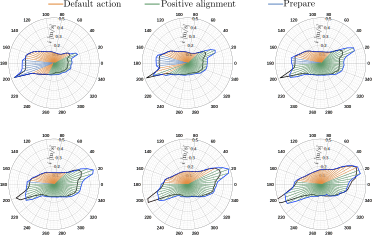
\includegraphics[width=0.85\textwidth]{STYLESTUFF/rounActions.png}
    \caption{Polar plots of the maximum recoverable impulses $i$ (radius) for the default controller (black) and the vertical motion controller (blue) for pushes applied at different moments in single support. The colors of the radial lines show the actions used by the vertical motion control law.}
    \label{fig:roundPushActions}
\end{figure}
\begin{figure}
     \centering
        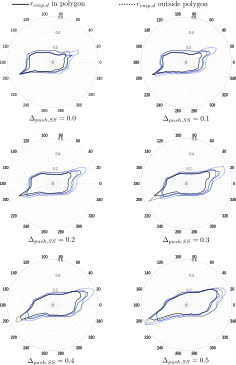
\includegraphics[width=0.85\textwidth]{STYLESTUFF/roundAng.png}
        \caption{Polar plots of the maximum recoverable impulses $i$ (radius) for the default controller (black) and vertical motion controller (blue). A comparison is shown for when the desired \ac{CMP} is constrained to be inside the polygon, and when the desired \ac{CMP} is allowed to leave the polygon $0.05$ [m].}
        \label{fig:roundPushAng}
\end{figure}

In \figref{fig:roundPushAng}, the maximum recoverable pushes are shown when $\rcmpd$ is constrained to be inside the polygon, like in the previous figure, and when $\rcmpd$ is allowed to leave the polygon $5$ [cm]. This distance outside the polygon is commonly used at \ac{IHMC} \cite{griffin2017natural}. Allowing $\rcmpd$ to leave the polygon requests angular momentum rate from the robot to achieve the desired linear momentum rate. However, how much of it is achieved is highly depending on the weights used in the whole-body \ac{QP}. Note how the plots with larger possible $\rcmpd$ locations seem to match shape with the plots where $\rcmpd$ is inside the polygon. Also note how for push directions coming from the back, the recovery is about the same for the default controller with larger $\rcmpd$ locations compared with the vertical motion controller where $\rcmpd$ is constrained to be inside the polygon.

\subsubsection{Comparison of Equal Push} 
A deeper evaluation is again made for the responses after an equal push for certain push directions. A rear and frontal push at the start of single support are chosen to make a deeper evaluation of, which have a recoverable impulse of $i=0.156$ [m/s] and $0.315$ [m/s] respectively. In \figref{fig:walkplot}, time responses are shown for these applied impulses. For the vertical motion controller, the positive alignment action is used for the rear push and the prepare action is used for the frontal push, which can also be observed in \figref{fig:roundPushActions}. For the back push, the desired vertical linear momentum rate $\dotldz$ from a circle is clearly visible after the second `bang'. The maximum height violates the maximum allowed height for the controller slightly halfway single support. For the prepare action however, the minimum height of the trajectory stays above the minimum height constraint. From the reference and measured \ac{ICP} $\icpr$ and $\icp$ in the sagittal direction, it can be observed that the final \ac{ICP} error is smaller for the vertical motion controller.
\begin{figure}
     \centering
        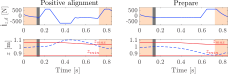
\includegraphics[width=0.99\textwidth]{STYLESTUFF/walkplot.png}
    \caption{Time responses after a rear push of $i=0.156$ [m/s] and a frontal push of $0.315$ [m/s] are applied on Valkyrie for both control setups. The push is applied in the dark gray area and the light gray area shows when the robot is in double support.}
    \label{fig:walkplot}
\end{figure}

\subsection{Atlas Hardware}
Additionally, some hardware tests on Atlas are conducted, triggering the positive alignment action. These tests are conducted on Atlas, as Atlas is able to walk faster than Valkyrie due to its more powerful actuation. Walking faster allows for \ac{CoM} positions at further distance from the \ac{CoP} positions, in which \ac{CoM} height variations have more effect on balance control. Unlike in the Valkyrie simulations, a step length of $0.4$ [m] is used. The same single support and double support times as in the Valkyrie simulations are used, which are about the maximum what the robot could do. In \figref{fig:walk3D}, the walking pattern and $\dotldz$ are depicted for the test. Intermediate local pendulums between $\rcmpd$ and the \ac{CoM} are depicted in the walking pattern after the push is applied with a constant time interval of $0.2$ [s]. The yellow lines show the projections on the $xz$-plane of the pendulums. The letters above the yellow lines match with letters below the images in \figref{fig:atw}; the pendulums are the $\rcmpd-\cxyz$ configurations for the images. At $a$ the push is applied and at $b$ released. The height change and the bang-bang control law of the positive alignment action are clearly visible. Instead of using the acceleration from a circle after the second `bang', a constant feedforward value is used on desired acceleration, because this was found to be simpler for tuning on the robot.
\begin{figure}
     \centering
        \includegraphics[width=0.99\textwidth]{STYLESTUFF/walk3D2.png}
        \caption{Visualization in \ac{3D} of the \ac{CoM} and $\rcmpd$ trajectory during the walking push recovery test (top). The yellow lines are the pendulums projected on the $xz$-plane. The letters above the yellow lines correspond with the letters below the images in \figref{fig:atw} and show the $\rcmpd$-$\cxyz$ configurations. At $a$, the push is applied and at $b$ the push is released. Also, $\dotldz$ over time is shown (bottom).}
        \label{fig:walk3D}
\end{figure}

\begin{figure}
\centering
  \begin{tabular}{cccc}
    \includegraphics[width=1.4in]{STYLESTUFF/atw4} &
    \includegraphics[width=1.4in]{STYLESTUFF/atw3} &
    \includegraphics[width=1.4in]{STYLESTUFF/atw2p} &
    \includegraphics[width=1.4in]{STYLESTUFF/atw1p} \\
    $d$ & $c$ & $b$ & $a$ ~\\[2ex]
    \includegraphics[width=1.4in]{STYLESTUFF/atw8} &
    \includegraphics[width=1.4in]{STYLESTUFF/atw7} &
    \includegraphics[width=1.4in]{STYLESTUFF/atw6} &
     \includegraphics[width=1.4in]{STYLESTUFF/atw5} \\
     $h$ & $g$ & $f$ & $e$ ~\\[2ex]
    \includegraphics[width=1.4in]{STYLESTUFF/atw12} &
    \includegraphics[width=1.4in]{STYLESTUFF/atw11} &
    \includegraphics[width=1.4in]{STYLESTUFF/atw10} &
    \includegraphics[width=1.4in]{STYLESTUFF/atw9} \\
    $l$ & $k$ & $j$ & $i$ 
  \end{tabular}
  \caption{Time-lapse of Atlas recovering from a push using the positive alignment action. The letters below the columns match with the corresponding letters above the yellow lines in \figref{fig:atw}. The push rod tip is encircled in red.}
  \label{fig:atw}
\end{figure}
% Discussion
\section{Discussion}
In this chapter, the control law of Chapter \ref{chap:standing} is extended for the use in \ac{3D}, using predefined strategies that can be heuristically be selected. These strategies rely on the predefined step time and location used in the control framework. Like in the previous chapter, control actions are chosen based on the violation of certain thresholds. 

The effective distance $\delta$ and the alignment angle $\phi$ allow for making a heuristic decision for the use of height control in different configurations. These variables are depending on the already existing \ac{ICP} control law. Based on these variables, a control action is introduced. Any misalignment with the error would result in additional error when using \ac{CoM} height variation for balance. This error is controlled with with future $\rcmpd$ positions. It could be interesting to already adjust for these additional errors by modifying $\rcmpd$ in advance.

From the results obtained for the step time and length considered, it seemed that height control in the beginning of single support results in the most improvement compared to strategies that do not use \ac{CoM} height variation. The vertical motion controller performs worse than the default setup around the $200$ degree push direction for all push moments in swing considered. This may be a results of the chosen control actions based on the thresholds $\phimin$, $\phimax$ and $\deltamin$, which are constant.

For the Atlas tests on hardware, the control law was difficult to compare to the default setup, and therefore there is chosen to only show an example of a result using the vertical motion controller. For the standing tests, it is assumed that the direction orthogonal to the push is constrained and the recovery problem is in \ac{2D}. For the walking test, the \ac{CoM} is located outside the support polygon if the push is applied and can also move orthogonal to the push direction. Furthermore, the robot is moving while the push is applied. Any small difference in the moment when the push is applied, the push location or the push direction can make a large difference in how the robot recovers. Therefore, a reliable comparison with the default setup on hardware for the walking tests could not be made and might be interesting to consider in the future. 
